\chapter{TorTella Application}
In questo capitolo si parlerà del funzionamento dell'applicazione realizzata e di tutti i suoi meccanismi. L'argomento è incentrato su: bootstrap, flooding, failure detection, invio e ricezione pacchetti, gestione pacchetti, concorrenza ed altro.
\section{BootStrap}
Il primo argomento riguarda il \textit{BootStrap} dell'applicazione, ovvero le operazioni effettuate per connettersi alla rete \textit{TorTella}. Per effettuare quanto detto si è deciso di fornire ad ogni peer una lista di coppie \textit{ip port} a cui connettersi inizialmente. Il metodo per reperire tale lista è al momento manuale (vedi \ref{conclusioni}). Le operazioni effettuate sono:
\begin{enumerate}
\item Viene avviata l'applicazione;
\item L'Applicazione prende un nodo dalla lista (ip e porta);
\item Avvia un \textit{client thread} che andrà a gestire l'invio di pacchetti verso il peer selezionato;
\item Il \textit{client thread} appena lanciato invierà inizialmente un pacchetto Ping (con fake recv\_ID), verso il peer a cui è associato, per stabilire la connessione;
\item Il peer ricevente risponde con un pacchetto di conferma e poi invia un Ping con il suo vero ID;
\item Il peer locale riceve il Ping e invia la conferma;
\item Connessione stabilita quindi torna al passo 2;
\end{enumerate}
Da questo elenco di azioni si può notare che avviene un invio del pacchetto Ping con fake recv\_ID, questo viene fatto perchè il peer locale che vuole entrare in TorTella Network non conosce l'ID dei nodi già presenti. Questo meccanismo di connessione che consente ai peer esterni alla rete di collegarsi senza problemi (vedi figura \ref{bootstrap}).
\begin{figure}[H]
\begin{center}
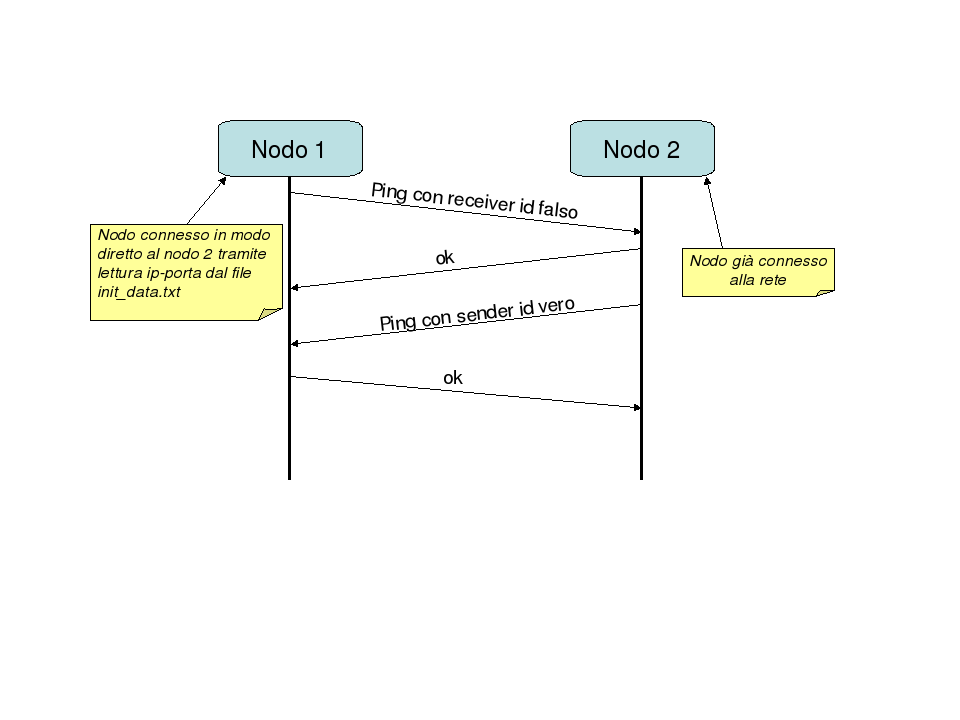
\includegraphics[scale=0.5]{etc/Bootstrap_conn.png}
\caption{BootStrap peer}
\label{bootstrap}
\end{center}
\end{figure}